\chapter{Introduction}
\label{introduction}
The centralization of power on Internet platforms cause unfairness in many industries. The technological advancements of the Internet has mainly lead to income polarization. The explosive increase in revenue on Internet platforms has mainly lead to higher profit margins for Big Tech instead of the core contributors on these platforms. During the last decades, we observe the trend of \textit{platformization}: a shift of economic activity from happening on a wide range of companies to a few major platforms run by Big Tech corporations. 
% Add a few numbers, or a graph showing hard facts on the rise of platformization
This trend is highly susceptible to the rise of monopolies and oligarchs.  This results in small and untraceable payouts to the core contributors on such platforms. The users of centralized platforms are affected by decisions that are made based on business strategies instead of democratic procedures.

Platformization already has a strong effect on the music industry, in which the succesful music streaming services have an immense amount of power. The biggest streaming services dictate the rules which artists have to play by. The top 5 streaming services and the top 3 labels dominate the market.
% Add exact percentages of market domination
Artists have a hard time to make a living because the streaming companies and labels take large revenue cuts of up to 40\%. The processing of royalties through many intermediaries is unclear on purpose. Artists can also suffer from political interference in these companies, reducing their freedom of speech. This thesis aims to distribute the power from centralized streaming platforms to listeners and artists, with the goals that artists (1) obtain a fair income and (2) are freed from censorship. 
\\
\\
The main contributions of this thesis are:
\begin{enumerate}
    \item A novel framework as an alternative for Big Tech: the robot economy in software;
    \item A partial implementation of this framework: a fully decentralized Android music streaming application \textit{MusicDAO} which attempts to liberate artists and consumers from powerful intermediaries.
\end{enumerate}
\\
MusicDAO implements a few key components of our framework: P2P leaderless infrastructure, resilient communication, trustless content sharing/exploration and a trustless monetary system (see \ref{tab:robot-economy-building-blocks}). The table shows that the other components of our robot economy framework, that are out of scope for this thesis, are under active experimentation and research by other scientists. We design, implement and evaluate the MusicDAO system. We perform controlled experiments with 10 Android devices to test the responsiveness and latency of its main features. Additionally, we release the application publicly to 50+ users and measure the monetary flows from users to artists over time. 
% is 50+ correct?
It is available on Google Play\footnote{\url{https://play.google.com/store/apps/details?id=nl.tudelft.trustchain}} and its code is open source\footnote{\url{github.com/Tribler/trustchain-superapp/}}.

% Add key findings from Evaluation

% https://www.opendemocracy.net/en/can-europe-make-it/robot-economy-full-automation-work-future/

\section{Monopolization on the Internet}
The Internet is moving from a network of people to a sparse selection of platforms over which nearly all commerce is regulated. The consumer choice is diminishing due to the power of oligarchs and monopolies. A few Big Tech corporations are gaining increasing power in the the surface on which market exchange takes place. These corporations take a large cut in revenue streams which majorly affects income for creators of content and services. Examples are Uber, Ebay and Spotify. Revenue streams towards the core contributors on a platforms are opaque on purpose. The software and algorithms powering these platforms are also a black box to creators and consumers. Furthermore, users have negligible influence on the future of these platforms. As explained by \citep{stiglitz2019market}, the funcamental problem is the growing ``concentration of market power, which allows dominant firms to exploit their customers and squeeze their employees, whose own bargaining power and legal protections are being weakened'', while ``[...] CEOs and executives are extracting higher pay for themselves''.

\section{Towards a robot economy}
An alternative for Big Tech is building a robot economy in software. Our novel vision of a robot economy follows recent theoretical groundwork by \cite{arduengo2020robot}: In a robot economy, intelligent robots play a key role, by performing economic operations autonomously. Robot tasks are driven by artificial intelligence, and cooperate with humans. While robots already take an active part in society today, the key difference in this vision is that robots have internal funds (which may be money, tokens or other assets) and can perform transactions on their own. Our work sets the first steps towards a robot economy in software by building and evaluating a few key components of this theory. Software as a robot economy is a service that runs autonomously, with which humans interact. Humans can spend funds, perform decisions or interact with data, while the software is run by robots.

A robot economy in software can have large influence: it can replace a company, or even a full value chain, Our framework for a robot economy in software allows designing and implementing \textit{infrastructure for the common good}: software that is governed by its key users and contributors, and as such leads to more fairness on Internet platforms. In a traditional software system, a company decides the parameters and functions of software. The software is run on company infrastructure only, which creates central points of failure. In a software system in the robot economy, its parameters and functions are voted on by its user base in a democratic voting process. It is run on distributed infrastructure, so is not susceptible to central points of failure. Since to the introduction of blockchains and crypto-currency, this voting process can be automated and transparent. Robots make intelligent decisions based on data and value given by humans. Such an implementation can replace entire value chains of industries.

\begin{figure}
    \centering
    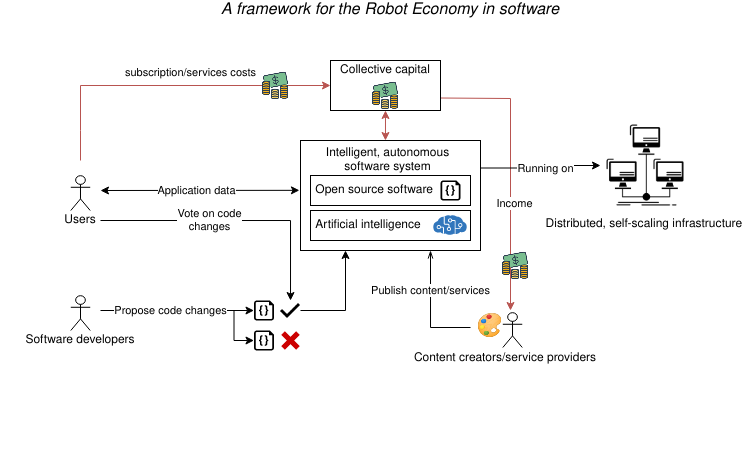
\includegraphics[width=1\textwidth]{introduction/robot-economy-2.png}
    \caption{A robot economy in software: democratic and autonomous software}
    \label{fig:robot-economy-in-software}
\end{figure}

As seen in \ref{fig:robot-economy-in-software}, the central component of the Robot Economy in software is an intelligent autonomous software system using a DAO. Every participant can vote on changes of the inner workings of the software using a democratic voting protocol. 

A full robot economy aims to have the following key characteristics: 
\begin{itemize}
    \item Automated;
    \item Transparent;
    \item Fair;
    \item Democratic;
    \item Open (permissionless);
    \item Leaderless;
    \item Self-evolving.
\end{itemize}
To accomplish these key characteristics in a software system, we envision the main building blocks to be as described in fig. \ref{tab:robot-economy-building-blocks}.

\section{Centralization of power in the music industry}
An industry with great consequences of this trend is the music industry. In the last 20 years there has been a remarkably fast shift from the exchange of CDs in various stores to music streaming on the Internet. Music platforms and labels use their economic muscle to push down artist salaries. They take large cuts of revenue from the user subscription money.

Firstly, corporations with power squeeze the music production side by taking large cuts of revenue from the user subscription money. As a result, the artists receive a low compensation. Especially independent artists have a hard time making a living. The distributors Spotify, iTunes and Google Play take on a 25\% to 40\% revenue cut.

Secondly, Big Tech has curatorial power to decide what is shown in the catalog of their application. The music catalog may seem endless, but in reality it is controlled by the Big Tech corporation and dictated by the interests of major labels. The inner workings of recommendation algorithms and playlists are in the hands of a few labels and streaming services.

Finally, the streaming companies can sensor tracks. The freedom of artist expression is then decided by undemocratic judgments. Big Tech has the power to decide the future of an artist.

\begin{figure}
    \centering
	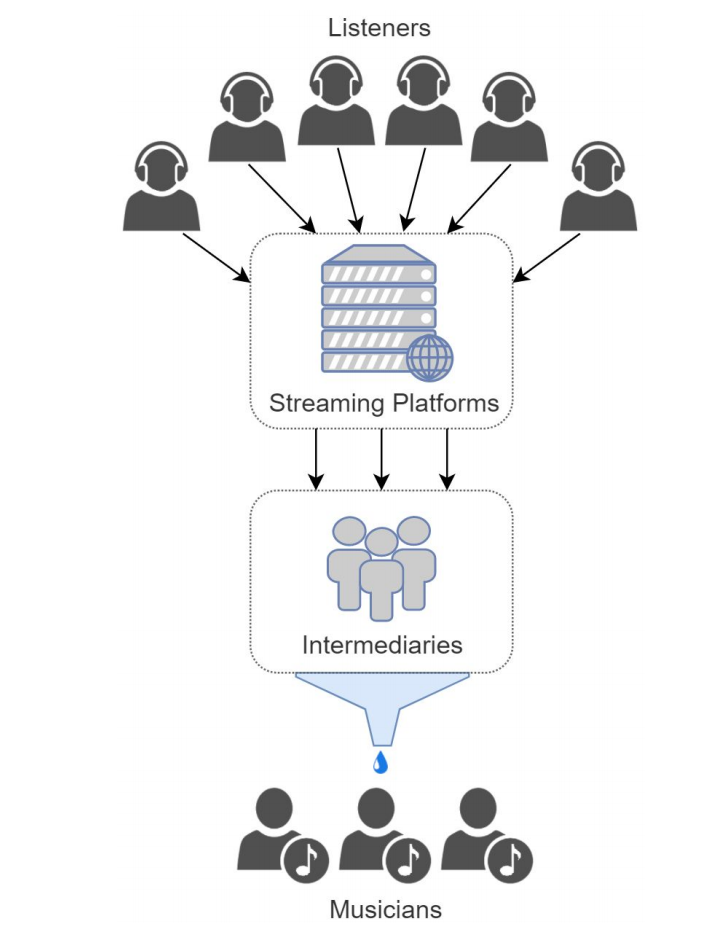
\includegraphics[width=0.4\textwidth]{introduction/problem-image.png}
	\caption{Artist compensation inconsistency}
\end{figure}

\section{Proposed solution: MusicDAO}
This thesis proposes an alternative technology from Big Tech streaming services. We observe that most functions of music streaming systems are already completely automated.
% Add a number: how much % is already automated?
We design and implement a decentralized system which attempts to replace the full value chain in music streaming industry, from the subscription money to the artist, by removing all intermediaries and giving power back to the artists and listeners. Listeners can stream music without being dependent on a single provider and can give money directly to artists. Artists receive 100\% of this donation and subscription money.

In essence, the solution is a decentralized autonomous organization (DAO) which is formed by listeners and artists. A DAO is defined by \cite{buterin2014dao} as an ``entity that lives on the internet and exists autonomously, but also heavily relies on hiring individuals to perform certain tasks that the automation itself cannot do'' (see \ref{fig:dao-quadrants}). In this thesis we present the design and implementation of our mobile android app MusicDAO: a music streaming service for the common good. Users of this app form a phone-to-phone zero-server network over which they publish music, download music and transfer money. This proof-of-principle of a DAO shows a fair and transparent music streaming service in which no external servers, third parties or intermediaries are necessary. Its operational network is leaderless and permissionless: any person can join, publish music and receive funds from peers. 100\% of music revenue goes to artists.

MusicDAO contains the following key functionalities:
\begin{itemize}
    \item Defining and publishing music content with metadata;
    \item Streaming music over BitTorrent;
    \item Caching and streaming optimization algorithms;
    \item Browsing playlists;
    \item Remote keyword search;
    \item Peer-to-peer donations to artists using Bitcoin.
\end{itemize}

In a real-world experiment with Android phones, we tested the feasibility of such a autonomous phone-to-phone system without centralized infrastructure. In a public release experiment, MusicDAO is published to the crowd via the Google Play Store\footnote{\url{https://play.google.com/store/apps/details?id=nl.tudelft.trustchain}}, and is installed on more than 50 devices. We evaluated all the money flow from its users towards the artists using a public blockchain. We evaluated the responsiveness of our decentralized infrastructure using supervised experiments, in which we measured the effect of network size on the latency of the key functionalities of our system.

\begin{table}[]
\centering
\begin{tabular}{|l|l|l|}
\hline
\textbf{Robot Economy component}                         & \textbf{Focus in MusicDAO} & \textbf{Related work} \\ \hline
Peer-to-peer leaderless and self-scaling infrastructure     & \checkmark  &                                    \\ \hline
Resilient communication                    & \checkmark  &                                    \\ \hline
Democratic user engagement                      &    & \cite{osgood2016future}, \cite{meter2017design}                                   \\ \hline
Trustless content sharing and exploration  & \checkmark &                                     \\ \hline
AI for decision making (robot tasks)       &   & \cite{dey2016machine}                                    \\ \hline
Trustless monetary system                  & \checkmark  &                                    \\ \hline

Continuous code evolution and distribution &   & \cite{jentzsch2016decentralized}, \cite{dupont2017experiments}                                     \\ \hline
\end{tabular}
\caption{The main components to achieve a robot economy in software}
\label{tab:robot-economy-building-blocks}
\end{table}
% Repeat this table in the Design section

% Most important: How can artists distribute and sell their work in a digital economy beholden to ruthlessly commercial and centralized interests?
% https://thebaffler.com/salvos/the-problem-with-muzak-pelly